\documentclass{standalone}
\usepackage{tikz}
\usepackage{ctex,siunitx}
\usepackage{tkz-euclide}
\usepackage{amsmath}
\usetikzlibrary{patterns, calc}
\usetikzlibrary {decorations.pathmorphing, decorations.pathreplacing, decorations.shapes,}
\begin{document}
\small
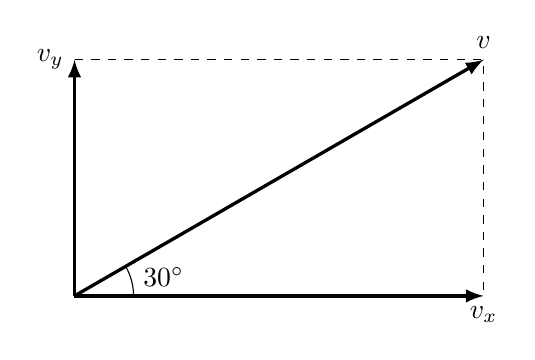
\begin{tikzpicture}[>=latex,scale=1.5]
  \draw [dashed](0,0) --(1.732*2,0) 
  --(1.732*2,2) --(0,2) ;
  \draw[->, very thick] (0,0)--(1.732*2,2)node [above]{$v$};
  \draw [->, very thick](0,0)--(1.732*2,0)node [below]{$v_x$};
  \draw [->, very thick](0,0)--(0,2)node [left]{$v_y$};
  \draw (0.5,0) arc(0:30:.5) node[at start,above right]{$\ang{30}$};
\end{tikzpicture}
\end{document}